\chapter{Control de la expresión génica}\label{ch:b1:expression-control}

Una bacteria que crece con glucosa lleva cinco moléculas de la \omterm{def:b1:enzymes:enzyme}{enzima} que
digiere la lactosa; dese le lactosa y, en minutos, llevará cinco mil. Una
\omterm{def:b1:cell-unit-of-life:cell}{célula} hepática y una \omterm{def:b1:body-plans-tissues:nervous}{neurona} llevan los mismos veinte mil \omterm{def:b1:genomes:gene}{genes} y fabrican
conjuntos de \omterm{def:b1:proteins:peptide}{proteínas} casi enteramente distintos, y ninguna fabricará nunca
el de la otra. Nada del \cref{ch:b1:gene-expression} explica esto: la
maquinaria de la expresión es la misma para todos los \omterm{def:b1:genomes:gene}{genes}. Lo que difiere
es si un \omterm{def:b1:genomes:gene}{gen} se lee, con qué frecuencia y durante cuánto tiempo: decisiones
que se toman en el promotor por \omterm{def:b1:proteins:peptide}{proteínas} que se unen al \omterm{def:b1:nucleic-acids:chain}{ADN} y, después de
él, por el destino del mensajero y de la \omterm{def:b1:proteins:peptide}{proteína}. Este capítulo describe
cómo las bacterias encienden y apagan \omterm{def:b1:genomes:gene}{genes} según su alimento, cómo los
eucariotas controlan los suyos mediante la cromatina, \omterm{def:b1:expression-control:enhancer}{potenciadores} lejanos
y combinaciones de factores, y cómo ese mismo control, aplicado a \omterm{def:b1:genomes:gene}{genes}
distintos en \omterm{def:b1:cell-unit-of-life:cell}{células} distintas, hace un cuerpo a partir de un solo \omterm{def:b1:genomes:genome}{genoma}.

\section{Por qué y dónde se controlan los genes}

\begin{proposition}[La expresión se regula, y en todos los niveles]\label{prop:b1:expression-control:levels}
\index{regulación génica}\index{gen constitutivo}
Algunos \omterm{def:b1:genomes:gene}{genes} son \emph{constitutivos}: se expresan siempre, y a un nivel
constante, porque sus productos son siempre necesarios (las \omterm{def:b1:proteins:peptide}{proteínas} del
\omterm{def:b1:gene-expression:ribosome}{ribosoma}, las \omterm{def:b1:enzymes:enzyme}{enzimas} de la \omterm{def:b1:respiration-fermentation:glycolysis}{glucólisis}). Casi todos están \emph{regulados}:
se expresan solo en ciertas condiciones, en ciertas \omterm{def:b1:cell-unit-of-life:cell}{células} y en ciertos
momentos. El control actúa en todos los pasos del flujo --- sobre todo al
comienzo de la transcripción, el lugar más barato donde decidir, pero
también en la maduración, la exportación, la estabilidad y la traducción del
mensajero, y en la modificación y la degradación de la \omterm{def:b1:proteins:peptide}{proteína} --- y los
tiempos de respuesta van de segundos (una \omterm{def:b1:proteins:peptide}{proteína} modificada) a minutos (un
\omterm{def:b1:genomes:gene}{gen} bacteriano encendido) y a días (un estado de cromatina cambiado).
\end{proposition}

\begin{example}[Fabricar enzimas solo cuando hacen falta]\label{ex:b1:expression-control:economy}
La \omterm{def:b1:enzymes:enzyme}{enzima} $\beta$-galactosidasa, que escinde la lactosa, es un tetrámero de
cuatro cadenas de \qty{1024}{} residuos: cinco mil copias son el
\qty{3}{\%} de la \omterm{def:b1:proteins:peptide}{proteína} de una \omterm{def:b1:cell-unit-of-life:cell}{célula} y cuestan \qty{8e7}{} \omterm{def:b1:water-small-molecules:atp}{ATP} por
generación. Una bacteria que las fabricara sin lactosa que digerir crecería
alrededor de un uno por ciento más despacio que una competidora que no lo
hiciera y, en unos cientos de generaciones, quedaría en minoría. La
regulación se selecciona porque la expresión es cara.
\end{example}

\section{El operón lac}

\begin{definition}[Operón, represor, operador]\label{def:b1:expression-control:operon}
\index{operón}\index{represor}\index{operador}\index{operón lac}
Un \emph{operón} es un grupo de \omterm{def:b1:genomes:gene}{genes} bacterianos que se transcriben juntos
desde un mismo promotor en un solo mensajero y que, por tanto, se controlan
juntos. El \emph{operón lac} de \emph{E. coli} comprende tres \omterm{def:b1:genomes:gene}{genes} para el
uso de la lactosa --- \emph{lacZ} ($\beta$-galactosidasa), \emph{lacY} (la
permeasa de lactosa que la importa) y \emph{lacA} --- tras un promotor y un
\emph{operador}, una secuencia corta que solapa con el promotor. Un \omterm{def:b1:genomes:gene}{gen}
aparte, \emph{lacI}, fabrica el \emph{represor lac}, una \omterm{def:b1:proteins:peptide}{proteína} que se une
al operador y bloquea la polimerasa. La lactosa, convertida en la \omterm{def:b1:cell-unit-of-life:cell}{célula} en
alolactosa, es el \emph{inductor}: se une al represor, le cambia la forma y
hace que suelte el operador. El operón está así apagado a menos que haya
lactosa: un \emph{control negativo} que levanta la \emph{inducción}.
\end{definition}

\begin{omfigure}
\begin{tikzpicture}[font=\footnotesize, >=Stealth, line cap=round]
  % state 1: no lactose
  \begin{scope}
    \draw[very thick, gray] (0,0) -- (11,0);
    \fill[omExo!50] (0.2,-0.2) rectangle (1.6,0.2); \node[anchor=south, font=\scriptsize] at (0.9,0.25) {\emph{lacI}};
    \fill[omProp!50] (2.4,-0.2) rectangle (3.6,0.2); \node[anchor=north, font=\scriptsize] at (3.0,-0.25) {promotor};
    \fill[omThm!50] (3.6,-0.2) rectangle (4.4,0.2); \node[anchor=south, font=\scriptsize] at (4.0,0.25) {operador};
    \fill[omDef!60] (4.5,-0.2) rectangle (7.2,0.2); \node[anchor=south, font=\scriptsize] at (5.85,0.25) {\emph{lacZ}};
    \fill[omDef!60] (7.3,-0.2) rectangle (9.0,0.2); \node[anchor=south, font=\scriptsize] at (8.15,0.25) {\emph{lacY}};
    \fill[omDef!60] (9.1,-0.2) rectangle (10.3,0.2); \node[anchor=south, font=\scriptsize] at (9.7,0.25) {\emph{lacA}};
    \node[draw, thick, fill=omThm!25, rounded corners=3pt, inner sep=2pt] (rep) at (4.0,-0.95) {represor};
    \draw[->, thick] (0.9,-0.25) -- (0.9,-0.95) -- (3.3,-0.95);
    \draw[thick] (rep) -- (4.0,-0.22);
    \node[draw, thick, fill=omProp!25, rounded corners=3pt, inner sep=2pt] at (2.2,0.9) {ARN polimerasa};
    \node[font=\scriptsize, anchor=west] at (3.45,0.9) {bloqueada};
    \node[anchor=east, align=right] at (-0.2,0) {sin lactosa:\\ operón APAGADO};
  \end{scope}
  % state 2: lactose present
  \begin{scope}[yshift=-3.0cm]
    \draw[very thick, gray] (0,0) -- (11,0);
    \fill[omExo!50] (0.2,-0.2) rectangle (1.6,0.2);
    \fill[omProp!50] (2.4,-0.2) rectangle (3.6,0.2);
    \fill[omThm!50] (3.6,-0.2) rectangle (4.4,0.2);
    \fill[omDef!60] (4.5,-0.2) rectangle (7.2,0.2); \fill[omDef!60] (7.3,-0.2) rectangle (9.0,0.2); \fill[omDef!60] (9.1,-0.2) rectangle (10.3,0.2);
    \node[draw, thick, fill=omThm!25, rounded corners=3pt, inner sep=2pt] (rep2) at (4.0,-1.0) {represor + inductor};
    \node[font=\scriptsize, anchor=west] at (5.6,-1.0) {liberado del operador};
    \node[draw, thick, fill=omProp!25, rounded corners=3pt, inner sep=2pt] at (3.0,0.85) {ARN polimerasa};
    \draw[->, very thick, omProp!80!black] (4.0,0.85) -- (10.3,0.85) node[midway, above, font=\scriptsize] {un mensajero para los tres genes};
    \node[anchor=east, align=right] at (-0.2,0) {con lactosa:\\ operón ENCENDIDO};
  \end{scope}
\end{tikzpicture}

{\small El \omterm{def:b1:expression-control:operon}{operón lac}. Sin lactosa el \omterm{def:b1:expression-control:operon}{represor} se sienta sobre el \omterm{def:b1:expression-control:operon}{operador} y
la polimerasa no puede arrancar; con lactosa el inductor aparta al \omterm{def:b1:expression-control:operon}{represor}
y los tres \omterm{def:b1:genomes:gene}{genes} se transcriben en un solo mensajero.}
\end{omfigure}

\begin{proposition}[El modelo del operón]\label{prop:b1:expression-control:jacobmonod}
Los \omterm{def:b1:genomes:gene}{genes} lac los controla un \omterm{def:b1:expression-control:operon}{represor} difusible que actúa sobre un sitio
contiguo a los \omterm{def:b1:genomes:gene}{genes}: el control es negativo, el \omterm{def:b1:expression-control:operon}{represor} actúa en
\emph{trans} (desde cualquier punto de la \omterm{def:b1:cell-unit-of-life:cell}{célula}) y el \omterm{def:b1:expression-control:operon}{operador} actúa en
\emph{cis} (solo sobre los \omterm{def:b1:genomes:gene}{genes} contiguos a él).
\end{proposition}
\begin{proof}[Evidencia]
Jacob y Monod (1959--1961) razonaron a partir de mutantes. Las cepas mutantes
en \emph{lacI} ($I^-$) fabricaban la \omterm{def:b1:enzymes:enzyme}{enzima} con lactosa o sin ella
(\emph{constitutivas}); un \omterm{def:b1:genomes:gene}{gen} \emph{lacI} normal introducido en una segunda
copia de la región restablecía la regulación, luego el producto del \omterm{def:b1:genomes:gene}{gen} es
un \omterm{def:b1:expression-control:operon}{represor} difusible del que un mutante carece. Las cepas mutantes en el
\omterm{def:b1:expression-control:operon}{operador} ($O^c$) también eran constitutivas, pero un segundo \omterm{def:b1:expression-control:operon}{operador} normal
en otra copia no restablecía la regulación: el \omterm{def:b1:expression-control:operon}{operador} solo controla los
\omterm{def:b1:genomes:gene}{genes} que tiene físicamente unidos, así que es un sitio y no un producto.
Una tercera clase ($I^s$) no podía inducirse en absoluto y era dominante: un
\omterm{def:b1:expression-control:operon}{represor} que ya no fija el inductor. En el experimento PaJaMo (1959), un \omterm{def:b1:genomes:gene}{gen}
\emph{lacI} normal transferido por conjugación a una \omterm{def:b1:cell-unit-of-life:cell}{célula} $I^-$ detuvo la
síntesis de la \omterm{def:b1:enzymes:enzyme}{enzima} en pocos minutos: el \omterm{def:b1:expression-control:operon}{represor} actúa deprisa y sobre la
transcripción; después se demostró que el mensajero tiene una vida media de
minutos.
\end{proof}

\begin{definition}[Control positivo: la CAP y el AMPc]\label{def:b1:expression-control:cap}
\index{represión catabólica}\index{diauxia}
El promotor lac es débil: incluso sin el \omterm{def:b1:expression-control:operon}{represor}, la polimerasa arranca
pocas veces si no hay una segunda \omterm{def:b1:proteins:peptide}{proteína}, la \emph{CAP} (\omterm{def:b1:proteins:peptide}{proteína}
activadora por catabolito), unida justo aguas arriba, que dobla el \omterm{def:b1:nucleic-acids:chain}{ADN} y
sujeta la polimerasa en su sitio. La CAP se une al \omterm{def:b1:nucleic-acids:chain}{ADN} solo cuando lleva
\emph{AMP cíclico}, cuyo nivel en la \omterm{def:b1:cell-unit-of-life:cell}{célula} cae cuando abunda la glucosa. El
\omterm{def:b1:expression-control:operon}{operón} está, por tanto, plenamente encendido solo cuando hay lactosa
\emph{y} falta glucosa: dos señales, una negativa y otra positiva, se
integran en un solo promotor. Con los dos azúcares presentes, \emph{E. coli}
consume primero la glucosa, hace una pausa mientras sube el AMPc y se
fabrican las \omterm{def:b1:enzymes:enzyme}{enzimas} lac, y consume después la lactosa: la curva de
crecimiento en dos fases llamada \emph{diauxia}, que Monod describió en 1941
y que lo puso en el camino del \omterm{def:b1:expression-control:operon}{operón}.
\end{definition}

\begin{omfigure}
\begin{tikzpicture}
\begin{semilogyaxis}[
  width=0.86\linewidth, height=6.0cm,
  axis x line=bottom, axis y line=left,
  xmin=0, xmax=6, ymin=1e7, ymax=3e9,
  xlabel={tiempo (h)}, ylabel={células por mL},
  xlabel style={font=\small, at={(axis description cs:0.5,-0.12)}, anchor=north},
  ylabel style={font=\small},
  tick label style={font=\small}, xtick={0,1,2,3,4,5,6},
  clip=false,
]
\addplot[very thick, omDef, domain=0:2, samples=30] {1e7*2^(x/0.333)};
\addplot[very thick, omDef, domain=2:2.6, samples=5] {6.4e8};
\addplot[very thick, omDef, domain=2.6:4.0, samples=30] {6.4e8*2^((x-2.6)/0.5)};
\addplot[very thick, omDef, domain=4.0:6, samples=5] {6.4e8*2^(1.4/0.5)};
\node[font=\scriptsize, anchor=north west, align=left] at (axis cs:0.15,8e8) {fase 1: glucosa\\ (duplicación \qty{20}{min})};
\node[font=\scriptsize, anchor=south, align=center] at (axis cs:2.3,7e8) {latencia: sube el AMPc,\\ se fabrican las enzimas lac};
\node[font=\scriptsize, anchor=north west, align=left] at (axis cs:3.0,9e8) {fase 2: lactosa\\ (duplicación \qty{30}{min})};
\node[font=\scriptsize, anchor=south west] at (axis cs:4.1,4.4e9) {};
\end{semilogyaxis}
\end{tikzpicture}

{\small Crecimiento diáuxico de \emph{E. coli} con glucosa y lactosa. El
cultivo crece solo con glucosa, se detiene cuando esta se agota y se reanuda
con lactosa tras la media hora que cuesta inducir el \omterm{def:b1:expression-control:operon}{operón lac}.}
\end{omfigure}

\begin{omfigure}
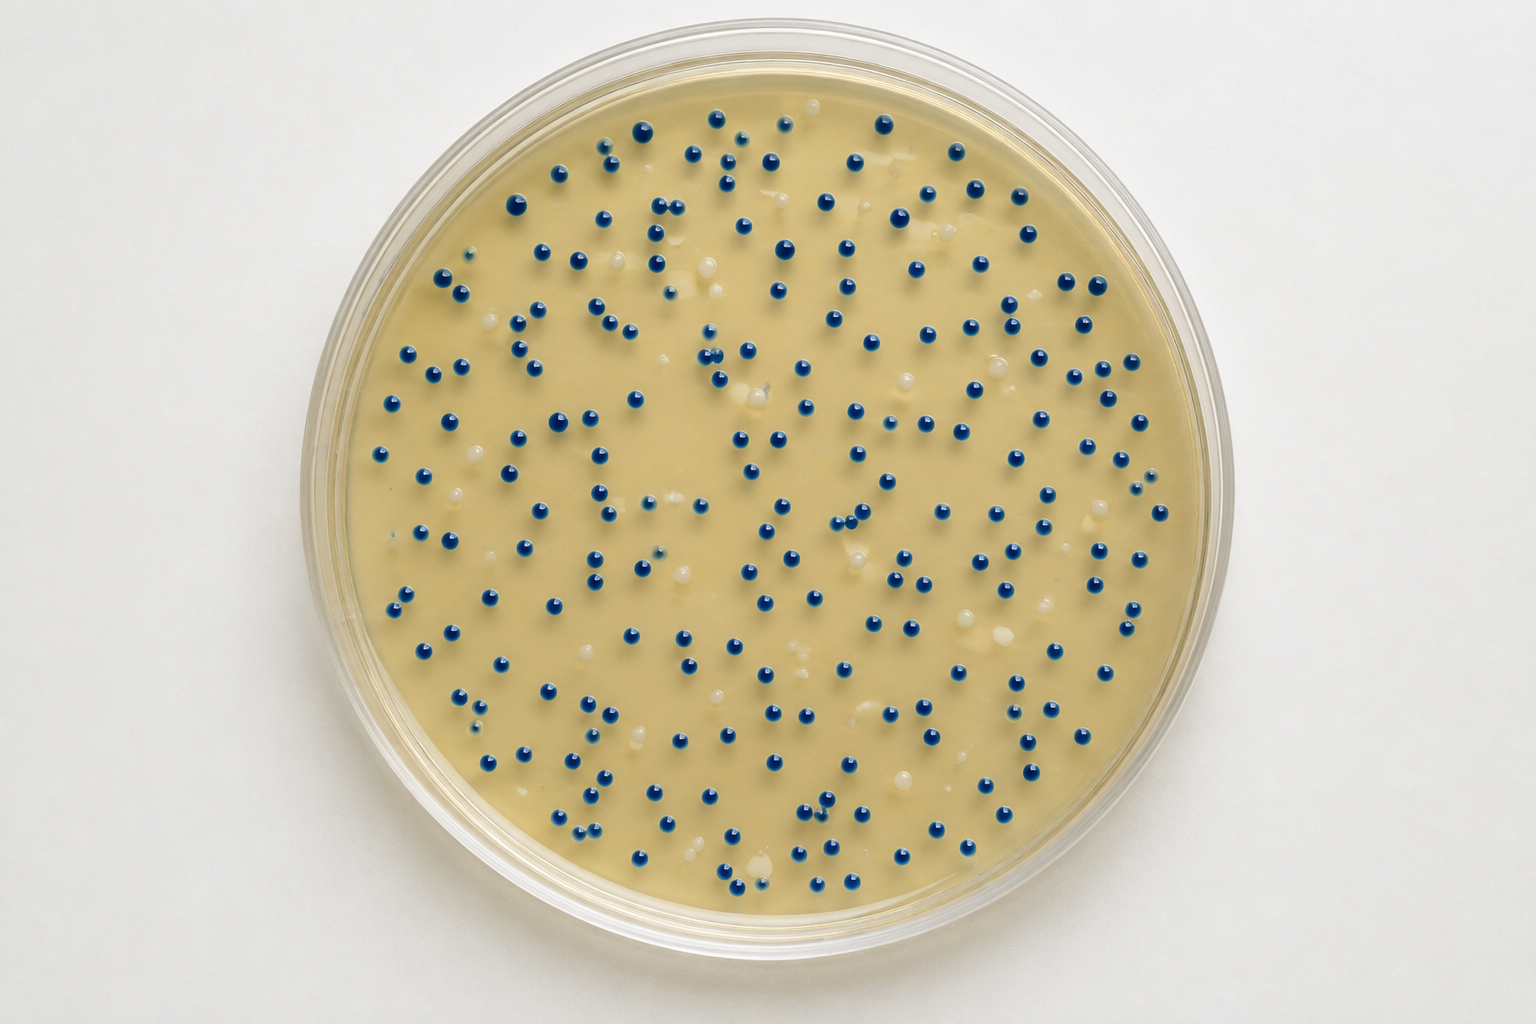
\includegraphics[width=0.46\linewidth]{images/book3/ai/b3-20-xgal-plate.png}

{\small El \omterm{def:b1:expression-control:operon}{operón lac} hecho visible: colonias en una placa con X-gal, un
\omterm{def:b1:enzymes:enzyme}{sustrato} incoloro que la $\beta$-galactosidasa vuelve azul. Las colonias
azules expresan \emph{lacZ}; las blancas llevan un \omterm{def:b1:genomes:gene}{gen} roto: el \omterm{def:b1:genomes:gene}{gen} delator
usado en mil experimentos.}
\end{omfigure}

\begin{method}[Predicción de un fenotipo lac]\label{met:b1:expression-control:lacphenotype}
\begin{enumerate}
  \item Escríbase el genotipo de cada copia de la región: $I$, $P$, $O$,
        $Z$ ($^+$ normal, $^-$ inactivo, $O^c$ \omterm{def:b1:expression-control:operon}{operador} constitutivo,
        $I^s$ superrepresor).
  \item El \omterm{def:b1:expression-control:operon}{represor} actúa en trans: un solo $I^+$ en cualquier sitio reprime
        todos los \omterm{def:b1:expression-control:operon}{operadores} normales; $I^s$ reprime haya el inductor que
        haya.
  \item El \omterm{def:b1:expression-control:operon}{operador} y el promotor actúan en cis: un $O^c$ libera solo el
        $Z$ de su propio \omterm{def:b1:nucleic-acids:chain}{ADN}; un $P^-$ silencia solo sus propios \omterm{def:b1:genomes:gene}{genes}.
  \item Pregúntese, con inductor y sin él, si cada \omterm{def:b1:genomes:gene}{gen} $Z^+$ se transcribe;
        el fenotipo será inducible, constitutivo o no inducible según el
        caso. Añádase después glucosa: sin AMPc--CAP la transcripción es
        baja haga lo que haga el \omterm{def:b1:expression-control:operon}{represor}.
\end{enumerate}
\end{method}

\begin{example}[Dos diploides parciales]\label{ex:b1:expression-control:diploids}
$I^-\,O^+\,Z^+ / I^+\,O^+\,Z^-$: la copia $I^+$ fabrica \omterm{def:b1:expression-control:operon}{represor} que se une
al $O^+$ contiguo a $Z^+$; inducible, pues la mutación queda complementada.
$I^+\,O^c\,Z^+ / I^+\,O^+\,Z^-$: el único $Z$ funcional está tras un
\omterm{def:b1:expression-control:operon}{operador} al que el \omterm{def:b1:expression-control:operon}{represor} no puede unirse; constitutivo, pues el \omterm{def:b1:expression-control:operon}{operador}
normal de la otra copia no puede ayudar, ya que solo controla el $Z$ roto.
\end{example}

\section{Otras estrategias bacterianas}

\begin{proposition}[Represión, atenuación y factores sigma]\label{prop:b1:expression-control:trp}
\index{operón trp}\index{atenuación}\index{factor sigma}
Los operones de biosíntesis se controlan en el sentido opuesto: el
\emph{\omterm{prop:b1:expression-control:trp}{operón trp}}, cinco \omterm{def:b1:genomes:gene}{genes} para fabricar triptófano, se transcribe a
menos que haya triptófano; el \omterm{def:b1:proteins:aminoacid}{aminoácido} se une al \omterm{def:b1:expression-control:operon}{represor} trp y lo
\emph{habilita} para unirse al \omterm{def:b1:expression-control:operon}{operador} (es un correpresor). Un segundo
control, más fino, la \emph{atenuación}, aprovecha el acoplamiento entre
transcripción y traducción de las bacterias: el comienzo del mensajero
codifica un péptido corto con dos triptófanos seguidos; si abunda el ARNt
cargado de triptófano, un \omterm{def:b1:gene-expression:ribosome}{ribosoma} lo traduce deprisa y el \omterm{def:b1:nucleic-acids:chain}{ARN} de detrás se
pliega en una horquilla terminadora que detiene la polimerasa antes de los
\omterm{def:b1:genomes:gene}{genes}; si el triptófano escasea, el \omterm{def:b1:gene-expression:ribosome}{ribosoma} se atasca en los codones de
triptófano y el \omterm{def:b1:nucleic-acids:chain}{ARN} se pliega de otro modo, con lo que la transcripción
continúa. Las bacterias cambian además conjuntos enteros de \omterm{def:b1:genomes:gene}{genes} cambiando
la subunidad $\sigma$ de su polimerasa: un $\sigma$ de choque térmico la
dirige a los promotores de los \omterm{def:b1:genomes:gene}{genes} de \omterm{prop:b1:proteins:denaturation}{chaperonas}; un $\sigma$ de
esporulación, a los de la formación de esporas.
\end{proposition}

\section{El control en los eucariotas}

\begin{definition}[Factores de transcripción, potenciadores]\label{def:b1:expression-control:enhancer}
\index{factor de transcripción}\index{potenciador}
En los eucariotas la polimerasa nunca arranca sola: los factores generales
del promotor (\cref{ch:b1:gene-expression}) la reclutan, y la velocidad la
fijan los \emph{factores de transcripción} unidos a \emph{secuencias
reguladoras} --- unas cercanas al promotor y muchas en
\emph{potenciadores} que pueden quedar a miles de \omterm{thm:b1:nucleic-acids:helix}{pares de bases}, aguas
arriba, aguas abajo o en un \omterm{def:b1:genomes:gene}{intrón}, en cualquier orientación, y que actúan
formando un \emph{bucle} en el \omterm{def:b1:nucleic-acids:chain}{ADN} para que los factores unidos a ellos
toquen el complejo del promotor a través de \omterm{def:b1:proteins:peptide}{proteínas} mediadoras. Un factor
de transcripción es modular: un \emph{dominio de unión al \omterm{def:b1:nucleic-acids:chain}{ADN}} que reconoce
una secuencia corta (familias hélice-giro-hélice, dedo de cinc, cremallera
de leucinas) y un dominio de \emph{activación} o de \emph{represión} que
recluta o bloquea la maquinaria. Un \omterm{def:b1:genomes:gene}{gen} se lee cuando está presente la
\emph{combinación} adecuada de factores: unos pocos cientos de factores, en
combinaciones, controlan veinte mil \omterm{def:b1:genomes:gene}{genes}.
\end{definition}

\begin{omfigure}
\begin{tikzpicture}[font=\footnotesize, >=Stealth, line cap=round]
  % DNA with enhancer far upstream, looped to promoter
  \draw[very thick, gray] (0,0) -- (2.2,0) .. controls (3.2,0) and (3.4,2.6) .. (5.0,2.6) .. controls (6.6,2.6) and (6.8,0) .. (7.8,0) -- (12.5,0);
  \fill[omExo!60] (0.4,-0.2) rectangle (2.0,0.2); \node[anchor=north, font=\scriptsize] at (1.2,-0.25) {potenciador (a \qtyrange{1}{100}{kb})};
  \fill[omProp!50] (8.0,-0.2) rectangle (9.4,0.2); \node[anchor=north, font=\scriptsize] at (8.7,-0.25) {promotor};
  \fill[omDef!60] (9.5,-0.2) rectangle (12.3,0.2); \node[anchor=north, font=\scriptsize] at (10.9,-0.25) {gen};
  % looped enhancer brought near promoter: draw factors at the loop apex near promoter? Simplify: activators on enhancer, mediator bridging
  \node[draw, thick, fill=omExo!30, rounded corners=3pt, inner sep=2pt] (act) at (1.2,0.75) {activadores};
  \node[draw, thick, fill=omThm!25, rounded corners=3pt, inner sep=2pt, align=center] (med) at (5.0,1.5) {mediador};
  \node[draw, thick, fill=omProp!30, rounded corners=3pt, inner sep=2pt, align=center] (pol) at (8.7,0.85) {factores generales\\ + polimerasa};
  \draw[thick, omExo!80!black] (act) -- (2.4,1.2) -- (med);
  \draw[thick, omThm] (med) -- (pol);
  \node[anchor=north, align=center, gray] at (6.2,-1.0) {el ADN forma un bucle para que los factores unidos lejos toquen el complejo del promotor;\\ un gen se lee cuando está unida la combinación adecuada de factores};
\end{tikzpicture}

{\small La acción de un \omterm{def:b1:expression-control:enhancer}{potenciador}. Los activadores unidos a un \omterm{def:b1:expression-control:enhancer}{potenciador}
lejano se acercan al promotor gracias a un bucle del \omterm{def:b1:nucleic-acids:chain}{ADN}, y un complejo
mediador transmite su señal a la polimerasa.}
\end{omfigure}

\begin{proposition}[La cromatina forma parte del control]\label{prop:b1:expression-control:chromatin}
\index{acetilación de histonas}\index{metilación del ADN}
Un \omterm{def:b1:genomes:gene}{gen} envuelto en \omterm{def:b1:genomes:nucleosome}{nucleosomas} empaquetados en heterocromatina no puede
leerse: los factores no llegan a él. Los activadores reclutan \omterm{def:b1:enzymes:enzyme}{enzimas} que
\emph{acetilan} las \omterm{def:b1:genomes:nucleosome}{histonas}, con lo que aflojan su agarre sobre el \omterm{def:b1:nucleic-acids:chain}{ADN} y
marcan la región como abierta; los \omterm{def:b1:expression-control:operon}{represores} reclutan \omterm{def:b1:enzymes:enzyme}{enzimas} que retiran
los grupos acetilo y añaden marcas que compactan la cromatina. Los grupos
metilo añadidos a las citosinas de un promotor lo silencian de manera
duradera, y las marcas se copian en la replicación, de modo que el patrón de
\omterm{def:b1:genomes:gene}{genes} abiertos y cerrados de una \omterm{def:b1:cell-unit-of-life:cell}{célula} lo heredan sus hijas: la memoria por
la que las hijas de una \omterm{def:b1:cell-unit-of-life:cell}{célula} hepática siguen siendo \omterm{def:b1:cell-unit-of-life:cell}{células} hepáticas (el
volumen del tercer año trata a fondo estos mecanismos \emph{epigenéticos}).
\end{proposition}
\begin{proof}[Evidencia]
En los \omterm{def:b1:genomes:genome}{cromosomas} politénicos gigantes de las larvas de mosca (mil copias de
cada \omterm{def:b1:genomes:genome}{cromosoma} una junto a otra, con bandas), los \omterm{def:b1:genomes:gene}{genes} que se están
transcribiendo aparecen como \emph{abultamientos} donde la cromatina se ha
desplegado; la hormona ecdisona, que desencadena la muda, hace aparecer un
conjunto concreto de abultamientos en pocos minutos y otros horas después,
en una secuencia fija: la transcripción vista directamente y accionada por
una señal. Los \omterm{def:b1:genomes:gene}{genes} desplazados por reordenaciones cromosómicas junto a la
heterocromatina quedan silenciados en unas \omterm{def:b1:cell-unit-of-life:cell}{células} y no en otras, y el
estado lo heredan sus hijas.
\end{proof}

\begin{omfigure}
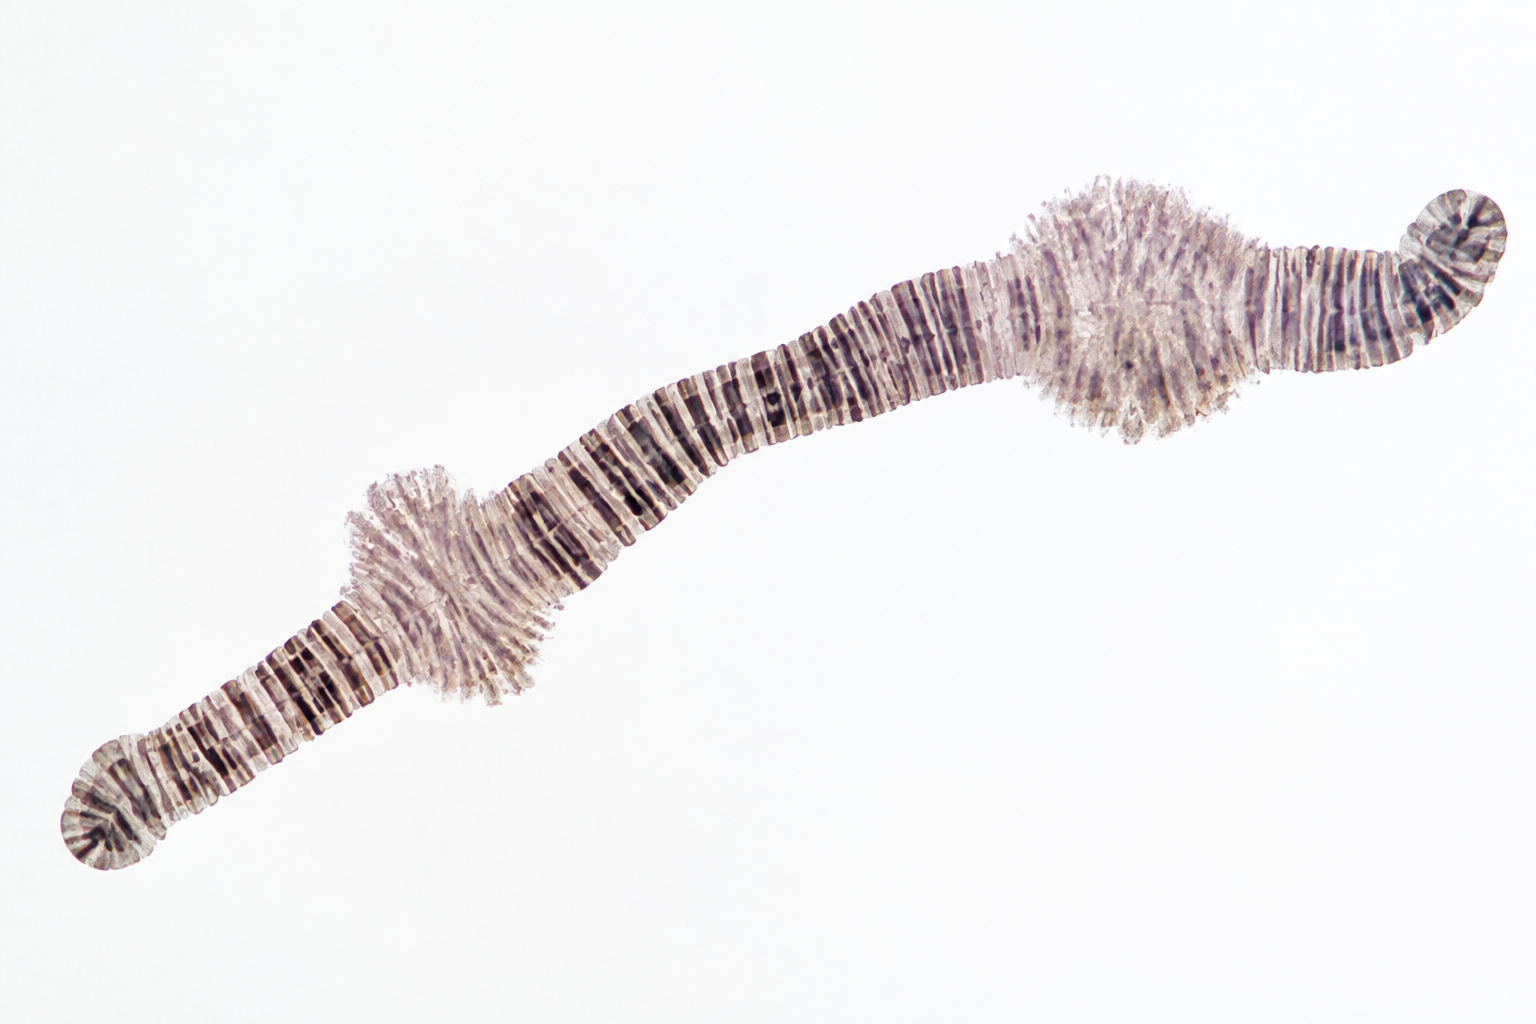
\includegraphics[width=0.56\linewidth]{images/book3/ai/b3-20-polytene-chromosome.png}

{\small Un \omterm{def:b1:genomes:genome}{cromosoma} politénico de la glándula salival de una mosca: con
bandas y con dos abultamientos donde la cromatina se ha abierto para la
transcripción. Los abultamientos aparecen y desaparecen a medida que los
\omterm{def:b1:genomes:gene}{genes} se encienden y se apagan.}
\end{omfigure}

\begin{example}[Una señal se convierte en un patrón de expresión]\label{ex:b1:expression-control:steroid}
El cortisol entra en una \omterm{def:b1:cell-unit-of-life:cell}{célula} hepática y se une a su receptor, un \omterm{def:b1:expression-control:enhancer}{factor
de transcripción} que se mantiene inactivo en el \omterm{def:b1:eukaryotic-cell:organelle}{citosol}; el complejo entra
en el núcleo, se une a una secuencia de quince bases presente cerca de un
centenar de \omterm{def:b1:genomes:gene}{genes} --- entre ellos los de la \omterm{def:b1:biosyntheses-integration:gluconeogenesis}{gluconeogénesis}
(\cref{ch:b1:biosyntheses-integration}) --- y recluta acetilasas y mediador:
en menos de una hora se están fabricando las \omterm{def:b1:enzymes:enzyme}{enzimas} de la síntesis de
glucosa. Esa misma hormona, en un linfocito cuya cromatina abierta expone un
conjunto distinto de esas secuencias, enciende \omterm{def:b1:genomes:gene}{genes} que matan a la \omterm{def:b1:cell-unit-of-life:cell}{célula}.
Una señal, un receptor, dos respuestas: la diferencia está en qué \omterm{def:b1:genomes:gene}{genes}
estaban accesibles.
\end{example}

\section{Después de la transcripción, y la construcción de un cuerpo}

\begin{proposition}[Control más allá del promotor]\label{prop:b1:expression-control:posttranscriptional}
\index{estabilidad del ARNm}
Una \omterm{def:b1:cell-unit-of-life:prokeuk}{célula eucariota} decide además cómo se corta y se empalma un transcrito
(el empalme alternativo da a un músculo y a un encéfalo \omterm{def:b1:proteins:peptide}{proteínas} distintas
a partir de un mismo \omterm{def:b1:genomes:gene}{gen}), si se exporta, cuánto dura (vidas medias que van
de minutos, en los mensajes de las \omterm{def:b1:proteins:peptide}{proteínas} reguladoras, a días, en el de
la hemoglobina, fijadas por secuencias de las regiones no traducidas que
unen \omterm{def:b1:proteins:peptide}{proteínas} y \omterm{def:b1:nucleic-acids:chain}{ARN} reguladores pequeños) y si se traduce (las \omterm{def:b1:cell-unit-of-life:cell}{células}
faltas de hierro bloquean la traducción del mensaje de la ferritina con una
\omterm{def:b1:proteins:peptide}{proteína} unida a su extremo $5'$, y la liberan cuando hay hierro). Una vez
fabricada, la \omterm{def:b1:proteins:peptide}{proteína} se controla por modificación y por degradación
(\cref{ch:b1:enzymes}). Cada nivel posterior es más rápido y más local que
el anterior, y más caro: la transcripción decide lo que la \omterm{def:b1:cell-unit-of-life:cell}{célula} puede
hacer, y los niveles posteriores lo que hace ahora.
\end{proposition}

\begin{proposition}[La expresión diferencial construye un cuerpo]\label{prop:b1:expression-control:differentiation}
\index{diferenciación}
Todas las \omterm{def:b1:cell-unit-of-life:cell}{células} de un \omterm{def:b1:organism-environment:organism}{organismo} pluricelular llevan el mismo \omterm{def:b1:genomes:genome}{genoma}; las
\omterm{def:b1:cell-unit-of-life:cell}{células} difieren porque expresan subconjuntos distintos de él. Los \omterm{def:b1:genomes:gene}{genes}
\emph{de mantenimiento} --- unos pocos miles, para el metabolismo, el
\omterm{def:b1:gene-expression:ribosome}{ribosoma} y el \omterm{def:b1:eukaryotic-cell:cytoskeleton}{citoesqueleto} --- están encendidos en todas las \omterm{def:b1:cell-unit-of-life:cell}{células}; los
demás se encienden en unas \omterm{def:b1:cell-unit-of-life:cell}{células} y se apagan en otras según las
combinaciones de \omterm{def:b1:expression-control:enhancer}{factores de transcripción} que lleve cada una y los estados
de cromatina que haya heredado. El precursor de un glóbulo rojo enciende la
globina y apaga casi todo lo demás; una \omterm{def:b1:body-plans-tissues:nervous}{neurona} enciende sus \omterm{def:b1:membranes-transport:transporters}{canales} y no
vuelve a dividirse. La \emph{diferenciación} es la adquisición de un patrón
estable de expresión, y el \emph{desarrollo} (volumen del segundo año) es el
proceso por el que las señales entre \omterm{def:b1:cell-unit-of-life:cell}{células} fijan esos patrones en los
lugares adecuados.
\end{proposition}
\begin{proof}[Evidencia]
Un núcleo tomado de una \omterm{def:b1:cell-unit-of-life:cell}{célula} diferenciada de rana y colocado en un óvulo
al que se ha retirado el suyo puede dirigir el desarrollo de un renacuajo
entero (Gurdon, 1962; recordado del volumen de bachillerato): la \omterm{def:b1:cell-unit-of-life:cell}{célula}
diferenciada no había perdido \omterm{def:b1:genomes:gene}{genes}, solo los había apagado, y el \omterm{def:b1:cell-unit-of-life:cell}{citoplasma}
del óvulo reajustó los interruptores. Las \omterm{def:b1:proteins:peptide}{proteínas} de un tipo celular,
separadas en un gel, difieren de las de otro tipo; sus mensajeros, una vez
secuenciados, son un subconjunto del \omterm{def:b1:genomes:genome}{genoma} propio de él; y un puñado de
\omterm{def:b1:expression-control:enhancer}{factores de transcripción} introducidos en una \omterm{def:b1:cell-unit-of-life:cell}{célula} de la piel pueden
reprogramarla como \omterm{def:b1:cell-unit-of-life:cell}{célula} madre o como \omterm{def:b1:body-plans-tissues:nervous}{neurona}.
\end{proof}

\begin{example}[Un gen leído en dos órganos]\label{ex:b1:expression-control:twoorgans}
El \omterm{def:b1:genomes:gene}{gen} de la \omterm{def:b1:enzymes:enzyme}{enzima} que fabrica glucosa a partir de glucosa-6-fosfato se
expresa en el hígado y en el riñón y en ningún otro \omterm{def:b1:body-plans-tissues:tissue}{tejido}: su promotor
lleva sitios para factores presentes solo allí, y en las demás \omterm{def:b1:cell-unit-of-life:cell}{células} ese
promotor está metilado y su cromatina cerrada. Un músculo, que lleva el \omterm{def:b1:genomes:gene}{gen}
intacto, no puede liberar glucosa a la sangre
(\cref{ch:b1:biosyntheses-integration}), no por falta del \omterm{def:b1:genomes:gene}{gen}, sino porque
el \omterm{def:b1:genomes:gene}{gen} no se lee. El \omterm{def:b1:genomes:genome}{genoma} es el mismo; la expresión es el \omterm{def:b1:mammal-organization:organ}{órgano}.
\end{example}

\section{Ejercicios}

\begin{exercise}[$\star$]\label{exo:b1:expression-control:1}
Nómbrense los elementos del \omterm{def:b1:expression-control:operon}{operón lac} y dese el estado del \omterm{def:b1:expression-control:operon}{operón} con
lactosa y sin ella, con glucosa y sin ella.
\end{exercise}

\begin{exercise}[$\star$]\label{exo:b1:expression-control:2}
Explíquese la diferencia entre un producto génico que actúa en trans y un
sitio que actúa en cis, con un ejemplo de cada uno del \omterm{def:b1:expression-control:operon}{operón}.
\end{exercise}

\begin{exercise}[$\star$]\label{exo:b1:expression-control:3}
A partir de la figura de la \omterm{def:b1:expression-control:cap}{diauxia}, léanse la duración de la latencia y los
tiempos de duplicación con cada azúcar.
\end{exercise}

\begin{exercise}[$\star$]\label{exo:b1:expression-control:4}
Defínanse \omterm{def:b1:expression-control:enhancer}{potenciador}, \omterm{def:b1:expression-control:enhancer}{factor de transcripción} y \omterm{def:b1:genomes:gene}{gen} de mantenimiento.
\end{exercise}

\begin{exercise}[$\star\star$]\label{exo:b1:expression-control:5}
Dese el fenotipo (inducible, constitutivo, no inducible) de: $I^-$;
$O^c$; $I^s$; $I^-\,O^+\,Z^+ / I^+\,O^+\,Z^+$; $I^s\,O^+\,Z^+ /
I^+\,O^+\,Z^+$; $I^+\,O^c\,Z^- / I^+\,O^+\,Z^+$.
\end{exercise}

\begin{exercise}[$\star\star$]\label{exo:b1:expression-control:6}
Compárense los operones lac y trp: qué le hace la molécula pequeña al
\omterm{def:b1:expression-control:operon}{represor} en cada uno, y por qué la lógica es opuesta.
\end{exercise}

\begin{exercise}[$\star\star$]\label{exo:b1:expression-control:7}
Un mutante no puede fabricar AMPc. Predíganse su crecimiento con glucosa,
con lactosa sola y con ambas, y el nivel de $\beta$-galactosidasa en cada
caso.
\end{exercise}

\begin{exercise}[$\star\star$]\label{exo:b1:expression-control:8}
Explíquese por qué la atenuación es imposible en los eucariotas, a partir de
la arquitectura de la \omterm{def:b1:cell-unit-of-life:prokeuk}{célula eucariota}.
\end{exercise}

\begin{exercise}[$\star\star$]\label{exo:b1:expression-control:9}
Un \omterm{def:b1:expression-control:enhancer}{potenciador} se traslada de \qty{5}{kb} aguas arriba de su \omterm{def:b1:genomes:gene}{gen} a
\qty{5}{kb} aguas abajo y se invierte; el \omterm{def:b1:genomes:gene}{gen} se sigue expresando.
Explíquese qué muestra esto sobre cómo funcionan los \omterm{def:b1:expression-control:enhancer}{potenciadores}.
\end{exercise}

\begin{exercise}[$\star\star\star$]\label{exo:b1:expression-control:10}
Cinco mil tetrámeros de $\beta$-galactosidasa de \qty{4096}{} residuos,
¿cuántos \omterm{def:b1:water-small-molecules:atp}{ATP} cuestan (cuatro por residuo)? El presupuesto de una \omterm{def:b1:cell-unit-of-life:cell}{célula} por
generación es de unos \qty{1e10}{} \omterm{def:b1:water-small-molecules:atp}{ATP}. Calcúlense la desventaja de
crecimiento de un mutante constitutivo y el número de generaciones que
tardaría su proporción en una población mixta en caer de la mitad a la
centésima parte.
\end{exercise}

\begin{exercise}[$\star\star\star$]\label{exo:b1:expression-control:11}
Se comparan una \omterm{def:b1:cell-unit-of-life:cell}{célula} hepática y una \omterm{def:b1:body-plans-tissues:nervous}{neurona} de la misma persona: mismo
\omterm{def:b1:genomes:genome}{genoma}, \omterm{def:b1:proteins:peptide}{proteínas} distintas, y cada división de la \omterm{def:b1:cell-unit-of-life:cell}{célula} hepática da
\omterm{def:b1:cell-unit-of-life:cell}{células} hepáticas. Explíquese, con la cromatina, los factores y la herencia
de las marcas, cómo se produce la diferencia y cómo se mantiene.
\end{exercise}

\begin{exercise}[$\star\star\star$]\label{exo:b1:expression-control:12}
``Una bacteria lee su entorno; una \omterm{def:b1:cell-unit-of-life:cell}{célula} de un cuerpo lee su historia.''
Discútanse en un párrafo los dos tipos de control, sus señales, sus escalas
de tiempo y su reversibilidad.
\end{exercise}

\section{Problema: la diauxia}

\begin{problem}[{Problema de fin de semana --- la curva de crecimiento en
dos fases de Monod reconstruida célula a célula: glucosa agotada, lactosa
inducida, enzimas contadas, mutantes predichos y el coste de la regulación
calculado, hasta llegar al factor de inducción de la
$\beta$-galactosidasa}]
\label{pb:b1:expression-control:1}
Un cultivo de \emph{E. coli} parte de $10^7$ \omterm{def:b1:cell-unit-of-life:cell}{células} por mililitro en un
medio con \qty{0.5}{mmol/L} de glucosa y \qty{1.0}{mmol/L} de lactosa. Con
glucosa las \omterm{def:b1:cell-unit-of-life:cell}{células} se duplican cada \qty{20}{min}, y con lactosa cada
\qty{30}{min}; una \omterm{def:b1:cell-unit-of-life:cell}{célula} necesita \qty{1.5e-12}{g} de azúcar por división
(\qty{180}{g/mol} de glucosa; la lactosa, \qty{342}{g/mol}, cuenta como dos
glucosas). Las \omterm{def:b1:cell-unit-of-life:cell}{células} no inducidas contienen 5 moléculas de
$\beta$-galactosidasa; plenamente inducidas, \num{5000}. La inducción tarda
\qty{30}{min}. La \omterm{def:b1:enzymes:enzyme}{enzima} es un tetrámero de $4\times 1024$ residuos; cada
residuo cuesta 4 \omterm{def:b1:water-small-molecules:atp}{ATP}; el presupuesto de \omterm{def:b1:water-small-molecules:atp}{ATP} de una \omterm{def:b1:cell-unit-of-life:cell}{célula} es de $10^{10}$
por división y su \omterm{def:b1:proteins:peptide}{proteína}, $\qty{1.5e-13}{g}$ (\qty{110}{Da} por residuo).

\medskip
\noindent\textbf{Parte I --- La fase de glucosa.}
\begin{enumerate}
  \item Calcúlese la glucosa disponible por mililitro, en gramos.
  \item ¿Cuántas divisiones por mililitro puede sostener?
  \item Partiendo de $10^7$ \omterm{def:b1:cell-unit-of-life:cell}{células}, ¿cuántas hay cuando se agota la
        glucosa? (Cada división produce una \omterm{def:b1:cell-unit-of-life:cell}{célula} nueva.)
  \item ¿Cuántas duplicaciones son, y cuánto dura la fase de glucosa?
  \item Durante esa fase, ¿en qué estado está el \omterm{def:b1:expression-control:operon}{operón lac}, y por qué, en
        términos moleculares (\omterm{def:b1:expression-control:operon}{represor} y CAP)?
\end{enumerate}

\medskip
\noindent\textbf{Parte II --- El cambio.}
\begin{enumerate}[resume]
  \item Cuando se acaba la glucosa, ¿qué sube dentro de las \omterm{def:b1:cell-unit-of-life:cell}{células} y a qué
        se une?
  \item La lactosa estuvo presente todo el tiempo. ¿Por qué, aun así, el
        \omterm{def:b1:expression-control:operon}{operón} estuvo casi apagado durante la fase de glucosa?
  \item Durante los \qty{30}{min} de latencia cada \omterm{def:b1:cell-unit-of-life:cell}{célula} fabrica sus
        \num{5000} \omterm{def:b1:enzymes:enzyme}{enzimas}. Calcúlense las moléculas de \omterm{def:b1:enzymes:enzyme}{enzima} fabricadas
        por segundo y por \omterm{def:b1:cell-unit-of-life:cell}{célula}, y los residuos por segundo.
  \item Una \omterm{def:b1:cell-unit-of-life:cell}{célula} contiene \num{20000} \omterm{def:b1:gene-expression:ribosome}{ribosomas} a \qty{20}{} residuos por
        segundo. ¿Qué fracción de su traducción dedica a la
        $\beta$-galactosidasa durante la latencia?
  \item Calcúlense la masa de \num{5000} tetrámeros y la fracción de la
        \omterm{def:b1:proteins:peptide}{proteína} de la \omterm{def:b1:cell-unit-of-life:cell}{célula} que representan.
  \item Calcúlese el factor de inducción.
  \item ¿Por qué es la permeasa (\emph{lacY}) tan necesaria como la \omterm{def:b1:enzymes:enzyme}{enzima}
        para crecer con lactosa, y qué le ocurre a un mutante
        \emph{lacY}$^-$ al que se da lactosa?
\end{enumerate}

\medskip
\noindent\textbf{Parte III --- La fase de lactosa.}
\begin{enumerate}[resume]
  \item Calcúlese la lactosa disponible por mililitro en equivalentes de
        glucosa, en gramos.
  \item ¿Cuántas divisiones más sostiene, y cuál es el recuento final de
        \omterm{def:b1:cell-unit-of-life:cell}{células}?
  \item ¿Cuánto dura la fase de lactosa?
  \item Establézcase la cronología: fase de glucosa, latencia, fase de
        lactosa, total.
  \item Explíquese por qué el tiempo de duplicación es mayor con lactosa
        (dos razones: una sobre el paso enzimático y otra sobre la
        permeasa).
\end{enumerate}

\medskip
\noindent\textbf{Parte IV --- Mutantes y costes.}
\begin{enumerate}[resume]
  \item Un mutante $I^-$: descríbanse su curva de crecimiento en ese mismo
        medio y su nivel de \omterm{def:b1:enzymes:enzyme}{enzima} a lo largo de ella.
  \item Un mutante CAP$^-$: descríbanse su curva y su nivel de \omterm{def:b1:enzymes:enzyme}{enzima}.
  \item Un mutante $O^c$ en un medio solo con lactosa: ¿hay alguna
        diferencia respecto del tipo silvestre? ¿Y en un medio solo con
        glucosa?
  \item Calcúlense el coste en \omterm{def:b1:water-small-molecules:atp}{ATP} por generación de fabricar \num{5000}
        tetrámeros y la fracción del presupuesto de la \omterm{def:b1:cell-unit-of-life:cell}{célula}.
  \item Si esa fracción alarga el tiempo de generación en esa misma
        proporción, ¿en cuánto queda el mutante $I^-$ por detrás del tipo
        silvestre en velocidad de crecimiento con glucosa?
  \item Partiendo de números iguales, ¿tras cuántas generaciones con
        glucosa es el mutante la décima parte de la población? ($r^n =
        0.1/0.9$, con $r$ el cociente de velocidades de crecimiento por
        generación, es decir, $2^{-\delta}$ para un retraso $\delta$ en
        duplicaciones.)
  \item Explíquese por qué, aun así, los mutantes $I^-$ son frecuentes en
        las cepas de laboratorio cultivadas con lactosa.
  \item Enúnciese el resultado: el factor de inducción de la
        $\beta$-galactosidasa, el coste de fabricarla innecesariamente como
        fracción del presupuesto de \omterm{def:b1:water-small-molecules:atp}{ATP}, y el tiempo total del experimento
        de \omterm{def:b1:expression-control:cap}{diauxia}.
\end{enumerate}
\end{problem}
